% Source: report/sections/02_dataset.md (owner: Janu, #3).
\section{Dataset}
\label{sec:data}

\subsection{Kvasir-SEG}
\label{sec:kvasir}
Kvasir-SEG~\cite{jha2020kvasir} contains \textbf{1000 colonoscopy images of polyps}, each with a pixel-level mask
in which white marks the polyp and black the background. The images were collected at Vestre Viken Health
Trust in Norway. The masks were drawn by a medical doctor and verified by an experienced gastroenterologist.
Image sizes vary from $332\times487$ to $1920\times1072$ pixels. Every image contains at least one polyp, and polyps differ
strongly in size, shape, colour and texture, which makes the dataset a realistic test of segmentation models.

\Cref{fig:samples} shows four test images from the smallest to the largest polyp,
with their ground-truth masks. In our test set, the polyp covers between 0.5\% and 71.9\% of the image
(median 11.7\%), and 27 of the 120 test images contain a small polyp (under 5\% of the image).

\begin{figure*}[t]
  \centering
  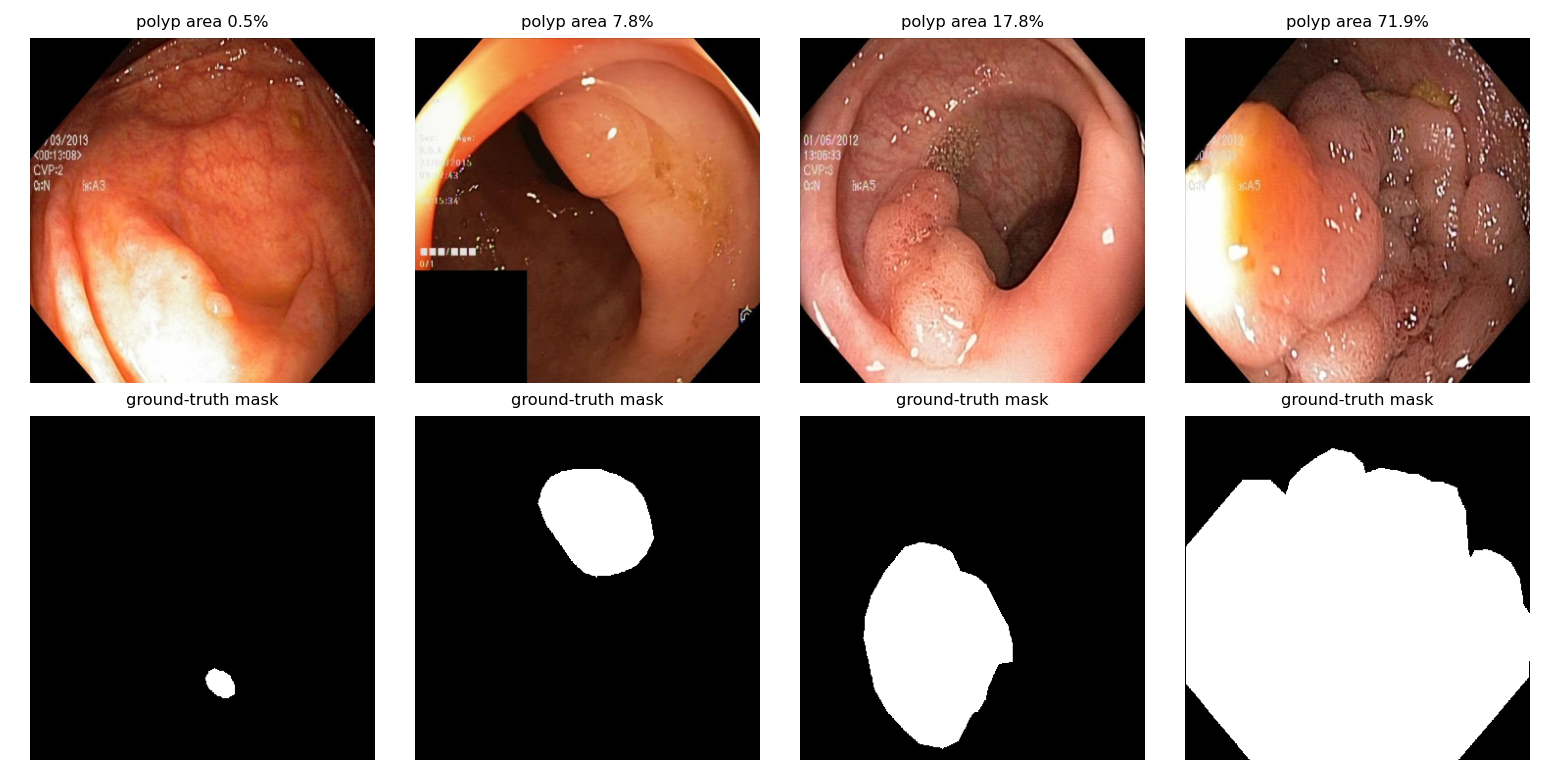
\includegraphics[width=0.78\textwidth]{dataset_samples.png}
  \caption{Four test images, from the smallest to the largest polyp, with their ground-truth masks.}
  \label{fig:samples}
\end{figure*}

\subsection{Split}
\label{sec:split}
We split the 1000 images once with a fixed random seed (42) into \textbf{800 training, 80 validation and
120 test images}. The test-set size follows the Kvasir-SEG paper; the split itself is our own. All five
models use exactly the same split, which is stored in \texttt{results/split.json}.
\begin{itemize}
  \item The \textbf{training set} is the only data the models learn from.
  \item The \textbf{validation set} is used for every choice made during development: keeping the best epoch
        and choosing the probability threshold.
  \item The \textbf{test set} is used only once per model, for the final numbers. It is never used to choose anything,
        so the reported scores are not optimistically biased.
\end{itemize}

\subsection{Preprocessing}
\label{sec:preproc}
Every image is resized to \textbf{$352\times352$ pixels}. Images use area interpolation, which keeps detail when
shrinking; masks use nearest-neighbour interpolation so they stay strictly binary. 352 is divisible by 16,
so the four $2\times2$ poolings of U-Net divide it exactly ($352 \rightarrow 176 \rightarrow 88 \rightarrow 44 \rightarrow 22$). Pixel values are scaled to
$[0, 1]$ and normalised with the ImageNet mean and standard deviation. The pretrained encoders were trained on
this normalisation, and we use it for all models so that the input is identical everywhere. The masks are
stored as JPEG files, so we threshold them at 127 to remove compression noise.

\subsection{Data augmentation}
\label{sec:augment}
With only 800 training images, the models would quickly memorise the training set. During training we
therefore apply random augmentations (\cref{tab:augment}), identically to the image and its mask, every time an image is loaded.
Validation and test images are never augmented.

\begin{table}[t]
  \centering
  \small
  \setlength{\tabcolsep}{3pt}
  \begin{adjustbox}{max width=\linewidth}
  \begin{tabular}{@{}p{0.27\linewidth}p{0.36\linewidth}p{0.33\linewidth}@{}}
    \toprule
    Augmentation & Setting & Why \\
    \midrule
    Horizontal and vertical flip & each with probability 0.5 & a colonoscope has no fixed ``up'' \\
    Rotation by a multiple of $90^\circ$ & uniform over $0^\circ$, $90^\circ$, $180^\circ$, $270^\circ$ & same reason, and it is lossless \\
    Rotation, scale and shift & probability 0.7: $\pm25^\circ$, scale 0.85--1.15, shift up to 6\% & changing camera angle and distance \\
    Brightness and contrast & probability 0.6: contrast $\times$0.8--1.2, brightness $\pm25$ & changing light and exposure \\
    \bottomrule
  \end{tabular}
  \end{adjustbox}
  \caption{Training augmentations, applied identically to the image and its mask.}
  \label{tab:augment}
\end{table}

\subsection{Additional evaluation data}
\label{sec:extra-data}
Two further datasets are used \textbf{only for evaluation}, never for training:
\begin{itemize}
  \item \textbf{Kvasir-Sessile}~\cite{jha2021sessile}: 196 of the Kvasir-SEG polyps that experts labelled as \textbf{sessile
        (flat) and smaller than 10\,mm}. We use it to tag the flat polyps in our test set (31 of the 120 test
        images) for the failure analysis.
  \item \textbf{CVC-ClinicDB}~\cite{bernal2015cvc}: 612 frames ($384\times288$ pixels) from 29 colonoscopy videos recorded at
        Hospital Cl\'{\i}nic in Barcelona, with expert masks. Because it comes from another hospital and another
        camera, it tests how well each model generalises beyond Kvasir-SEG.
\end{itemize}
